\documentclass[11pt]{article}

\usepackage{epsfig}
\usepackage{amsfonts}
\usepackage{amssymb}
\usepackage{amstext}
\usepackage{amsmath}
\usepackage{xspace}
\usepackage{theorem}
\usepackage{graphicx}
\usepackage{tikz}
\usepackage{pgfplots}

% \usepackage{layout}% if you want to see the layout parameters
% and now use \layout command in the body

% This is the stuff for normal spacing
\makeatletter
 \setlength{\textwidth}{6in}
 \setlength{\oddsidemargin}{0in}
 \setlength{\evensidemargin}{0.5in}
 \setlength{\topmargin}{0in}
 \setlength{\textheight}{9in}
 \setlength{\headheight}{0pt}
 \setlength{\headsep}{0pt}
 \setlength{\marginparwidth}{59pt}

 \setlength{\parindent}{0pt}
 \setlength{\parskip}{5pt plus 1pt}
 \setlength{\theorempreskipamount}{5pt plus 1pt}
 \setlength{\theorempostskipamount}{0pt}
 \setlength{\abovedisplayskip}{8pt plus 3pt minus 6pt}


\newenvironment{proof}{{\bf Proof:  }}{\hfill\rule{2mm}{2mm}}
\newenvironment{proofof}[1]{{\bf Proof of #1:  }}{\hfill\rule{2mm}{2mm}}
\newenvironment{proofofnobox}[1]{{\bf#1:  }}{}
\newenvironment{example}{{\bf Example:  }}{\hfill\rule{2mm}{2mm}}


\newtheorem{theorem}{Theorem}
\newtheorem{lemma}[theorem]{Lemma}
\newtheorem{proposition}[theorem]{Proposition}
\newtheorem{claim}[theorem]{Claim}
\newtheorem{corollary}[theorem]{Corollary}
\newtheorem{definition}[theorem]{Definition}

% math notation
\newcommand{\R}{\ensuremath{\mathbb R}}
\newcommand{\Z}{\ensuremath{\mathbb Z}}
\newcommand{\N}{\ensuremath{\mathbb N}}
\newcommand{\F}{\ensuremath{\mathbb F}}
\newcommand{\C}{\ensuremath{\mathbb C}}

\newcommand{\size}[1]{\ensuremath{\left|#1\right|}}
\newcommand{\ceil}[1]{\ensuremath{\left\lceil#1\right\rceil}}
\newcommand{\floor}[1]{\ensuremath{\left\lfloor#1\right\rfloor}}


% anupam's abbreviations
\newcommand{\mnote}[1]{\normalmarginpar \marginpar{\tiny #1}}


% vectors
\renewcommand{\vec}[1]{\ensuremath{\mathbf{#1}}}

\newenvironment{sol}
    {\emph{Solution:}
    }


%%%%%%%%%%%%%%%%%%%%%%%%%%%%%%%%%%%%%%%%%%%%%%%%%%%%%%%%%%%%%%%%%%%%%%%%%%%
% Document begins here %%%%%%%%%%%%%%%%%%%%%%%%%%%%%%%%%%%%%%%%%%%%%%%%%%%%
%%%%%%%%%%%%%%%%%%%%%%%%%%%%%%%%%%%%%%%%%%%%%%%%%%%%%%%%%%%%%%%%%%%%%%%%%%%


\newcommand{\headings}{
\large{\textbf{YOUR NAME GOES HERE \hfill 21-241 Fall 2019}\\
\textbf{Homework 6 \hfill Due Friday, October 11}}\\
\rule[0.1in]{\textwidth}{0.01in}
%\thispagestyle{empty}
}

\pagestyle{empty}

\begin{document}

\headings

\begin{enumerate}
\section*{Required Problems}
\item\label{gram} (Strang 4.4.18) Find orthogonal vectors $\vec{A}$, $\vec{B}$, $\vec{C}$ by Gram-Schmidt from $\vec{a}$, $\vec{b}$, $\vec{c}$:
\[\vec{a} = (1,-1,0,0) \quad \vec{b} = (0, 1, -1, 0) \quad \vec{c} = (0,0,1,-1).\]
$\vec{A}$, $\vec{B}$, $\vec{C}$ and $\vec{a}$, $\vec{b}$, $\vec{c}$ are bases for the vector space perpendicular to $\vec{d} = (1,1,1,1)$.

 \begin{sol}
Write your solution here.
\end{sol}
\clearpage


\item Let $A = \begin{bmatrix} 1 & 0 & 0 \\ -1 & 1  & 0 \\ 0 & -1 & 1 \\ 0 & 0 & -1 \end{bmatrix}$.  Write $A$ in the form $QR$, where $Q$ has orthonormal columns, and $R$ is upper triangular.  

Hint: Use results from Problem~\ref{gram}.


 \begin{sol}
Write your solution here.
\end{sol}
\clearpage

\item\label{ortho} (From Strang 4.4.10) In this problem you will prove that orthonormal vectors are automatically linearly independent in two ways (Note they are really the same proof, just written differently! --DO).
\begin{enumerate}
\item Vector proof: When $c_1 \vec{q}_1 + c_2 \vec{q}_2 + \cdots + c_n \vec{q}_n = \vec{0}$, what dot products lead to $c_1 = 0$?  Similarly $c_2 = 0$, and so forth.  Thus the $\vec{q}$'s are independent.
\item Matrix proof: Show that $Q\vec{x} = \vec{0}$ leads to $\vec{x} = \vec{0}$. Since $Q$ may be rectangular, you can use $Q^T$ but not $Q^{-1}$.
\end{enumerate}

 \begin{sol}
Write your solution here.
\end{sol}
\clearpage

\item Use the (7,4) Hamming code defined in class, with 
\[ H = \begin{bmatrix} 1 & 1 & 1 & 0 & 1 & 0 & 0 \\ 1& 1& 0 & 1& 0 & 1 & 0 \\1 & 0 & 1& 1& 0 &0 & 1\end{bmatrix}
\quad \text{ and } \quad
G = \begin{bmatrix} 1 & 0 & 0 & 0 \\ 0 & 1& 0 & 0 \\  0 &0 & 1 & 0 \\ 0 &  0 &0 & 1 \\ 1 & 1 & 1 & 0 \\ 1 & 1 & 0 & 1 \\ 1 & 0 & 1 & 1\end{bmatrix}
\]
to answer the following questions.
\begin{enumerate}
\item Suppose Alice wishes to encode the message $(0,0,1,0)$.  What is $C_A$?
\item Suppose Bob receives the message $C_B = (0,0,1,0,0, 1, 1)$.  What was the original message $M$?
\item Suppose Bob receives the message $C_B = (0,0,1,0,1, 1, 1)$.  What was the original message $M$?
\item Suppose Bob receives the message $C_B = (0,0,1,0,1, 0, 1)$.  What was the original message $M$?
\end{enumerate}

 \begin{sol}
Write your solution here.
\end{sol}
\clearpage


\item Define the \textit{Hamming distance} between two vectors in $\F_2^n$ to be the number of components in which they differ.  For example, the Hamming distance between $(0,1,0,0,1,1,1,0)$ and $(1,1,1,0,1,1,0,0)$ is three (components 1, 3, and 7 are different).  In this problem, we show that any two codewords in the Hamming code must have Hamming distance at least 3 from each other.
\begin{enumerate}
\item Show that two codewords in the (7,4) Hamming code cannot be at Hamming distance 1 from each other. 

Hint: Use the fact that if $C_1$ and $C_2$ are two codewords at distance 1 then for some $i$, $C_1 = C_2 + e_i$.
\item  Show that two codewords in the (7,4) Hamming code cannot be at Hamming distance 2 from each other. 

Hint: Use the fact that if $C_1$ and $C_2$ are two codewords at distance 2 then for some $i, j$, $C_1 = C_2 + e_i + e_j$.

\end{enumerate}

 \begin{sol}
Write your solution here.
\end{sol}
\clearpage

\item\label{digraph} Consider the following directed graph $D$.

\begin{center}
    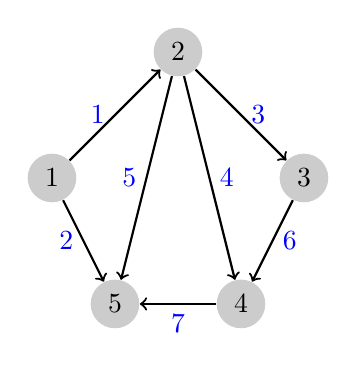
\begin{tikzpicture}[scale=.8]  
      \node[circle,fill=black!20] (v1) at (-1,1) {$1$};
      \node[circle,fill=black!20] (v2) at (1,3)  {$2$};
      \node[circle,fill=black!20] (v3) at (3,1) {$3$};
      \node[circle,fill=black!20] (v4) at (2,-1) {$4$};
     \node[circle,fill=black!20] (v5) at (0,-1) {$5$};
    \draw[thick,->] (v1) -- node[left] {\color{blue} 1} (v2) ;
   \draw[thick,->] (v1) --  node[left] {\color{blue} 2}  (v5);
    \draw[thick,->] (v2) -- node[right] {\color{blue} 3}  (v3) ;
   \draw[thick,->] (v2) --  node[right] {\color{blue} 4}  (v4);
    \draw[thick,->] (v2) --  node[left] {\color{blue} 5}  (v5);
  \draw[thick,->] (v3) --  node[right] {\color{blue} 6}  (v4);
   \draw[thick,->] (v4) --  node[below] {\color{blue} 7}  (v5);
    \end{tikzpicture}
\end{center}

\begin{enumerate}
\item What is the incidence matrix $A$ corresponding to $D$?  For grading purposes, please use the node and arc labels in order as given in the figure.
\item Use RREF to find a basis for the row space of $A$. You do not need to show each step of finding the RREF if you do not want to.
\item What is the spanning tree of $D$ corresponding to the basis in Part (b)?
\end{enumerate}

 \begin{sol}
Write your solution here.
\end{sol}
\clearpage

\item Consider the same digraph $D$ and adjacency matrix $A$ from Problem~\ref{digraph}.
\begin{enumerate}
\item Find the RREF for $A^T$, and use it to find a basis $\{\vec{v}_1, \vec{v}_2, \vec{v}_3\}$ for $N(A^T)$.
\item Find cycles $C_1$, $C_2$, and $C_3$ in $D$ corresponding to $\vec{v}_1$, $\vec{v}_2$, and $\vec{v}_3$, respectively.
\item Show that the cycle with arcs 1, 3, 6, 7, and 2 can be obtained from a linear combination of the vectors in the cycle basis.  Write the corresponding equation in terms of $\vec{v}_1$, $\vec{v}_2$, and $\vec{v}_3$.
\item Show that the cycle with arcs 5, 3, 6, and 7 can be obtained from a linear combination of the vectors in the cycle basis.  Write the corresponding equation in terms of $\vec{v}_1$, $\vec{v}_2$, and $\vec{v}_3$.
\item Let $T$ be the spanning tree from Problem~\ref{digraph}.  Show that each cycle in the cycle basis is obtained by taking the union of an arc $e$ not in $T$ with the arcs in $T$ connecting the endpoints of $e$. 

[This is an example of a general principle for generating a cycle basis of a connected graph: Given a spanning tree $T$, the cycles formed by adding a non-tree edge to $T$ form a cycle basis for the graph.  Note that this is consistent with the fact that the dimension of $N(A^T)$ is $n-m+1$ (Since the rank of $A$ is $n-1$, the dimension of the column space is $n-1$, so by the Rank-nullity theorem, $\dim N(A^T) = m-n+1$.)]
\end{enumerate}

 \begin{sol}
Write your solution here.
\end{sol}
\clearpage


\section*{Optional Problems}

\item Let $A$ be an $m \times n$ matrix with rank $r$. Suppose $V=\{\vec{v}_1, \ldots, \vec{v}_r\}$ is an orthonormal basis for $C(A^T)$ and $W=\{\vec{w}_1, \ldots, \vec{w}_{n-r}\}$ is an orthonormal basis for $N(A)$.  Use Problem~\ref{ortho} to give a simple proof that $V \cup W$ is a basis for $\R^n$.

\item Write Julia code to perform the Gram-Schmidt algorithm.

\item (Strang 4.4.33) Find all matrices that are both orthogonal and lower triangular.


\end{enumerate}


\end{document}